\chapter{前後の部分文書の情報の加味}

\section{前後の部分文書の情報}
NTCIR11のタスクでは,講演をより小さい単位で分割し,その一つを部分文書として,部分文書に対する検索精度を競う.部分文書に対して検索を行う場合,部分文書は文書長が短く,情報が少ないため,検索精度が低下すると考えられる.そのため本研究では,検索対象文書の周囲の文書も加味する事によって,文書検索精度の向上を図る.

% TODO: 先行研究との比較をしても良い

まず,クエリと $i$ 番目の部分文書との類似スコアを $Score(i)$ とおく.この部分文書に対し,$i-N$ から $i+N$ 番目の部分文書を考慮する時,$ Score’(i)$ は式(\ref{zengo1})で計算する.

\begin{equation}
    Score'(i) = \sum_{n=-N}^N w_n・Score(i + n) 
    \label{zengo1}
\end{equation}

ここで $w_n$は部分文書に付与する重みである.本研究では,適切な重みを調べるため,式(9.1)のnに応じた $w_n$ の変化が上に凸,比例,下に凸になるように,(i)ガウス重み,(ii)比例重み,(iii)反比例重みの3つを提案する.\\

{\bf(i)ガウス重み} \\

式(\ref{zengo1})の $n$ に応じて,ガウス関数を利用した重みを付与する.ガウス重みは,分散パラメータ $\sigma$ を用いて式(\ref{zengo2})で示す.

\begin{equation}
    w_n = \alpha⋅\exp⁡\{-(\frac{n}{2\sigma})^2\}
    \label{zengo2}
\end{equation}

ここで,$\alpha$ は $\sum_n w_n = 1$ となるように選ばれたスケールファクタである.また,分散パラメータ $\sigma$ は,部分文書の前後 $N$ 個を利用して式(\ref{zengo3})のように定義した.

\begin{equation}
    \sigma = 0.3 * (\frac{2N+1}{2}) - 1 + 0.8
    \label{zengo3}
\end{equation}

{\bf(ii)比例重み} \\

式(\ref{zengo1})の $n$ に応じて,比例的重みを付与する.比例重み $w_n$ を式(\ref{zengo4})で定義した.

\begin{equation}
    w_n = N+1-|n|
    \label{zengo4}
\end{equation}

{\bf(iii)反比例重み} \\

式(\ref{zengo1})の $n$ に応じて,反比例的重みを付与する.反比例重み $w_n$ を式(\ref{zengo5})で定義した.

\begin{equation}
    w_n = 
    \begin{cases} 
        1 & (i = 0)\\ 
        \frac{1}{|i|+1} & (|i| > 0)
    \end{cases} 
    \label{zengo5}
\end{equation}

\section{評価実験}
\subsection{実験条件}

{\Large TODO: 今回のNTCIR11 formal-runのクエリ・検索対象文書を音声認識結果ものを利用しやりなおし. \\
同様の結果になりそうなのは確認済み.}

前後の部分文書にガウス重み・比例重み・反比例重みを用い,スコアを統合したときのMAP値の変化と前後の部分文書の数を変えたときのMAP値の変化を示す.スムージングパラメータは,$\alpha= 0.5, \mu= 0.5, \nu= 0.0$ である.

\subsection{実験結果}
実験結果を図\ref{web_result1}に示す.

\begin{figure}[htbp]
    \centering
    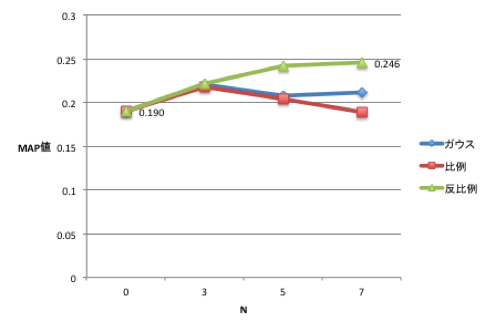
\includegraphics[width=7cm]{./image/zengo.png}
    \caption{前後の部分文書の加味したときのMAP値}
    \label{web_result1}
\end{figure}

実験結果として,図\ref{web_result1}から前後の部分文書を考慮するだけでもMAP値が上昇した.また,反比例重みを付与する事により,MAP値は最大0.246となり,前後の部分文書を考慮しないときよりもMAP値は0.056上昇した.この結果から,検索対象文書に対するスコアが重要であり,周囲の部分文書のスコアも少ない重みを付与して統合すると,検索精度が向上するといえる.

